\begin{statement}{1}
  Halle dos ra\'ices reales de $f(x) = |x^3| + x - 6$
  usando el m\'etodo de Newton. Use las aproximaciones
  iniciales $-1$ y $1$ y una exactitud de $10^{-4}$.
  Esboce la funci\'on usando MATLAB para verificar que la
  ecuaci\'on tiene solo dos ra\'ices.
\end{statement}

\begin{solution}
  Primero, realicemos la gr\'afica para obser que $f$ tiene dos ra\'ices.
  \begin{figure}[h!]
    \centering
    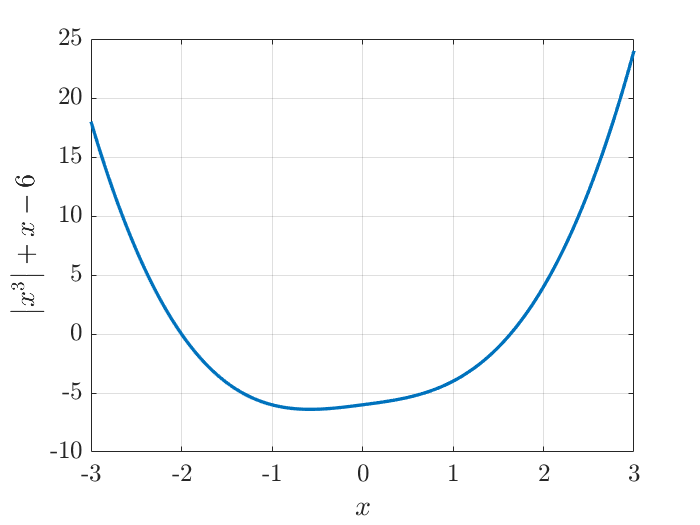
\includegraphics[scale=0.5]{plot-01.png}
    \caption{Esbozo de $f$}
  \end{figure}
  Analicemos la
\end{solution}